% Options for packages loaded elsewhere
\PassOptionsToPackage{unicode,linktoc=all}{hyperref}
\PassOptionsToPackage{hyphens}{url}
%
\documentclass[
  11pt,
  a4paper,
  nottoc]{report}

\usepackage{amsmath,amssymb}
\usepackage{setspace}
\usepackage{iftex}
\ifPDFTeX
  \usepackage[T1]{fontenc}
  \usepackage[utf8]{inputenc}
  \usepackage{textcomp} % provide euro and other symbols
\else % if luatex or xetex
  \usepackage{unicode-math}
  \defaultfontfeatures{Scale=MatchLowercase}
  \defaultfontfeatures[\rmfamily]{Ligatures=TeX,Scale=1}
\fi
\usepackage{lmodern}
\ifPDFTeX\else  
    % xetex/luatex font selection
\fi
% Use upquote if available, for straight quotes in verbatim environments
\IfFileExists{upquote.sty}{\usepackage{upquote}}{}
\IfFileExists{microtype.sty}{% use microtype if available
  \usepackage[]{microtype}
  \UseMicrotypeSet[protrusion]{basicmath} % disable protrusion for tt fonts
}{}
\usepackage{xcolor}
\usepackage[top=25mm,left=25mm,right=30mm,heightrounded,marginparwidth=1.5in,twoside=true]{geometry}
\setlength{\emergencystretch}{3em} % prevent overfull lines
\setcounter{secnumdepth}{2}

\usepackage{color}
\usepackage{fancyvrb}
\newcommand{\VerbBar}{|}
\newcommand{\VERB}{\Verb[commandchars=\\\{\}]}
\DefineVerbatimEnvironment{Highlighting}{Verbatim}{commandchars=\\\{\}}
% Add ',fontsize=\small' for more characters per line
\newenvironment{Shaded}{}{}
\newcommand{\AlertTok}[1]{\textcolor[rgb]{1.00,0.33,0.33}{\textbf{#1}}}
\newcommand{\AnnotationTok}[1]{\textcolor[rgb]{0.42,0.45,0.49}{#1}}
\newcommand{\AttributeTok}[1]{\textcolor[rgb]{0.84,0.23,0.29}{#1}}
\newcommand{\BaseNTok}[1]{\textcolor[rgb]{0.00,0.36,0.77}{#1}}
\newcommand{\BuiltInTok}[1]{\textcolor[rgb]{0.84,0.23,0.29}{#1}}
\newcommand{\CharTok}[1]{\textcolor[rgb]{0.01,0.18,0.38}{#1}}
\newcommand{\CommentTok}[1]{\textcolor[rgb]{0.42,0.45,0.49}{#1}}
\newcommand{\CommentVarTok}[1]{\textcolor[rgb]{0.42,0.45,0.49}{#1}}
\newcommand{\ConstantTok}[1]{\textcolor[rgb]{0.00,0.36,0.77}{#1}}
\newcommand{\ControlFlowTok}[1]{\textcolor[rgb]{0.84,0.23,0.29}{#1}}
\newcommand{\DataTypeTok}[1]{\textcolor[rgb]{0.84,0.23,0.29}{#1}}
\newcommand{\DecValTok}[1]{\textcolor[rgb]{0.00,0.36,0.77}{#1}}
\newcommand{\DocumentationTok}[1]{\textcolor[rgb]{0.42,0.45,0.49}{#1}}
\newcommand{\ErrorTok}[1]{\textcolor[rgb]{1.00,0.33,0.33}{\underline{#1}}}
\newcommand{\ExtensionTok}[1]{\textcolor[rgb]{0.84,0.23,0.29}{\textbf{#1}}}
\newcommand{\FloatTok}[1]{\textcolor[rgb]{0.00,0.36,0.77}{#1}}
\newcommand{\FunctionTok}[1]{\textcolor[rgb]{0.44,0.26,0.76}{#1}}
\newcommand{\ImportTok}[1]{\textcolor[rgb]{0.01,0.18,0.38}{#1}}
\newcommand{\InformationTok}[1]{\textcolor[rgb]{0.42,0.45,0.49}{#1}}
\newcommand{\KeywordTok}[1]{\textcolor[rgb]{0.84,0.23,0.29}{#1}}
\newcommand{\NormalTok}[1]{\textcolor[rgb]{0.14,0.16,0.18}{#1}}
\newcommand{\OperatorTok}[1]{\textcolor[rgb]{0.14,0.16,0.18}{#1}}
\newcommand{\OtherTok}[1]{\textcolor[rgb]{0.44,0.26,0.76}{#1}}
\newcommand{\PreprocessorTok}[1]{\textcolor[rgb]{0.84,0.23,0.29}{#1}}
\newcommand{\RegionMarkerTok}[1]{\textcolor[rgb]{0.42,0.45,0.49}{#1}}
\newcommand{\SpecialCharTok}[1]{\textcolor[rgb]{0.00,0.36,0.77}{#1}}
\newcommand{\SpecialStringTok}[1]{\textcolor[rgb]{0.01,0.18,0.38}{#1}}
\newcommand{\StringTok}[1]{\textcolor[rgb]{0.01,0.18,0.38}{#1}}
\newcommand{\VariableTok}[1]{\textcolor[rgb]{0.89,0.38,0.04}{#1}}
\newcommand{\VerbatimStringTok}[1]{\textcolor[rgb]{0.01,0.18,0.38}{#1}}
\newcommand{\WarningTok}[1]{\textcolor[rgb]{1.00,0.33,0.33}{#1}}

\providecommand{\tightlist}{%
  \setlength{\itemsep}{0pt}\setlength{\parskip}{0pt}}\usepackage{longtable,booktabs,array}
\usepackage{calc} % for calculating minipage widths
% Correct order of tables after \paragraph or \subparagraph
\usepackage{etoolbox}
\makeatletter
\patchcmd\longtable{\par}{\if@noskipsec\mbox{}\fi\par}{}{}
\makeatother
% Allow footnotes in longtable head/foot
\IfFileExists{footnotehyper.sty}{\usepackage{footnotehyper}}{\usepackage{footnote}}
\makesavenoteenv{longtable}
\usepackage{graphicx}
\makeatletter
\def\maxwidth{\ifdim\Gin@nat@width>\linewidth\linewidth\else\Gin@nat@width\fi}
\def\maxheight{\ifdim\Gin@nat@height>\textheight\textheight\else\Gin@nat@height\fi}
\makeatother
% Scale images if necessary, so that they will not overflow the page
% margins by default, and it is still possible to overwrite the defaults
% using explicit options in \includegraphics[width, height, ...]{}
\setkeys{Gin}{width=\maxwidth,height=\maxheight,keepaspectratio}
% Set default figure placement to htbp
\makeatletter
\def\fps@figure{htbp}
\makeatother
% definitions for citeproc citations
\NewDocumentCommand\citeproctext{}{}
\NewDocumentCommand\citeproc{mm}{%
  \begingroup\def\citeproctext{#2}\cite{#1}\endgroup}
\makeatletter
 % allow citations to break across lines
 \let\@cite@ofmt\@firstofone
 % avoid brackets around text for \cite:
 \def\@biblabel#1{}
 \def\@cite#1#2{{#1\if@tempswa , #2\fi}}
\makeatother
\newlength{\cslhangindent}
\setlength{\cslhangindent}{1.5em}
\newlength{\csllabelwidth}
\setlength{\csllabelwidth}{3em}
\newenvironment{CSLReferences}[2] % #1 hanging-indent, #2 entry-spacing
 {\begin{list}{}{%
  \setlength{\itemindent}{0pt}
  \setlength{\leftmargin}{0pt}
  \setlength{\parsep}{0pt}
  % turn on hanging indent if param 1 is 1
  \ifodd #1
   \setlength{\leftmargin}{\cslhangindent}
   \setlength{\itemindent}{-1\cslhangindent}
  \fi
  % set entry spacing
  \setlength{\itemsep}{#2\baselineskip}}}
 {\end{list}}
\usepackage{calc}
\newcommand{\CSLBlock}[1]{\hfill\break\parbox[t]{\linewidth}{\strut\ignorespaces#1\strut}}
\newcommand{\CSLLeftMargin}[1]{\parbox[t]{\csllabelwidth}{\strut#1\strut}}
\newcommand{\CSLRightInline}[1]{\parbox[t]{\linewidth - \csllabelwidth}{\strut#1\strut}}
\newcommand{\CSLIndent}[1]{\hspace{\cslhangindent}#1}

\usepackage{booktabs}
\usepackage{longtable}
\usepackage{array}
\usepackage{multirow}
\usepackage{wrapfig}
\usepackage{float}
\usepackage{colortbl}
\usepackage{pdflscape}
\usepackage{tabu}
\usepackage{threeparttable}
\usepackage{threeparttablex}
\usepackage[normalem]{ulem}
\usepackage{makecell}
\usepackage{xcolor}
\makeatletter
\@ifpackageloaded{bookmark}{}{\usepackage{bookmark}}
\makeatother
\makeatletter
\@ifpackageloaded{caption}{}{\usepackage{caption}}
\AtBeginDocument{%
\ifdefined\contentsname
  \renewcommand*\contentsname{Table of contents}
\else
  \newcommand\contentsname{Table of contents}
\fi
\ifdefined\listfigurename
  \renewcommand*\listfigurename{List of Figures}
\else
  \newcommand\listfigurename{List of Figures}
\fi
\ifdefined\listtablename
  \renewcommand*\listtablename{List of Tables}
\else
  \newcommand\listtablename{List of Tables}
\fi
\ifdefined\figurename
  \renewcommand*\figurename{Figure}
\else
  \newcommand\figurename{Figure}
\fi
\ifdefined\tablename
  \renewcommand*\tablename{Table}
\else
  \newcommand\tablename{Table}
\fi
}
\@ifpackageloaded{float}{}{\usepackage{float}}
\floatstyle{ruled}
\@ifundefined{c@chapter}{\newfloat{codelisting}{h}{lop}}{\newfloat{codelisting}{h}{lop}[chapter]}
\floatname{codelisting}{Listing}
\newcommand*\listoflistings{\listof{codelisting}{List of Listings}}
\makeatother
\makeatletter
\makeatother
\makeatletter
\@ifpackageloaded{caption}{}{\usepackage{caption}}
\@ifpackageloaded{subcaption}{}{\usepackage{subcaption}}
\makeatother
\ifLuaTeX
  \usepackage{selnolig}  % disable illegal ligatures
\fi
\usepackage{bookmark}

\IfFileExists{xurl.sty}{\usepackage{xurl}}{} % add URL line breaks if available
\urlstyle{same} % disable monospaced font for URLs
\hypersetup{
  pdftitle={This is my thesis},
  pdfauthor={Susan Su},
  hidelinks,
  pdfcreator={LaTeX via pandoc}}

%% CAPTIONS
\usepackage{caption}
\DeclareCaptionStyle{italic}[justification=centering]
 {labelfont={bf},textfont={it},labelsep=colon}
\captionsetup[figure]{style=italic,format=hang,singlelinecheck=true}
\captionsetup[table]{style=italic,format=hang,singlelinecheck=true}

%% FONT
\usepackage{bera}
\usepackage[charter]{mathdesign}
\usepackage[scale=0.9]{sourcecodepro}
\usepackage[lf,t]{FiraSans}
\usepackage{fontawesome}
%% IPA symbols
\usepackage{tipa}
%% underlining of title according to Uni Konstanz template
\usepackage{xcolor,soul}
\definecolor{seeblau}{HTML}{59C7EB}
\setulcolor{seeblau}
\setul{2pt}{2pt}% 1pt below contents

\usepackage[utf8]{inputenc}
%% HEADERS AND FOOTERS
% \usepackage{fancyhdr}
% \pagestyle{fancy}
% \rfoot{\Large\sffamily\raisebox{-0.1cm}{\textbf{\thepage}}}
% \makeatletter
% \lhead{\textsf{\expandafter{\@title}}}
% \makeatother
% \rhead{}
% \cfoot{}
% \setlength{\headheight}{15pt}
% \renewcommand{\headrulewidth}{0.4pt}
% \renewcommand{\footrulewidth}{0.4pt}
% \fancypagestyle{plain}{%
% \fancyhf{} % clear all header and footer fields
% \fancyfoot[C]{\sffamily\thepage} % except the center
% \renewcommand{\headrulewidth}{0pt}
% \renewcommand{\footrulewidth}{0pt}}
\usepackage{fancyhdr}
\usepackage{etoolbox}
\pagestyle{fancy}

% Clear all header and footer fields
\fancyhf{}

% Customizing the header for even and odd pages
\fancyhead[RO]{\textsf{\thepage}} % Page number on the right for odd pages
\fancyhead[LE]{\textsf{\thepage}} % Page number on the left for even pages
\fancyhead[LO]{\textsf{\nouppercase{\leftmark}}} % Chapter title on the left for odd pages
\fancyhead[RE]{\textsf{\nouppercase{\leftmark}}} % Chapter title on the right for even pages

% No footer customization needed since we are not displaying anything in the footer
\renewcommand{\footrulewidth}{0pt}

% Additional settings for plain pages (e.g., start of chapters)
\fancypagestyle{plain}{%
  \fancyhf{} % clear all header and footer fields
  \fancyfoot[C]{\textsf{\thepage}} % Page number centered in the footer with same font and size as header
  \renewcommand{\headrulewidth}{0pt} % No header rule
  \renewcommand{\footrulewidth}{0pt} % No footer rule
}

\setlength{\headheight}{15pt}
\renewcommand{\headrulewidth}{0.4pt}
\renewcommand{\footrulewidth}{0pt}

% Ensure the plain style is applied to chapter starting pages and switch to fancy after
\makeatletter
\preto\chapter{\clearpage\thispagestyle{plain}}
\patchcmd{\chapter}{\thispagestyle{plain}}{\thispagestyle{plain}\pagestyle{fancy}}{}{}
\makeatother


%% MATHS
\usepackage{bm,amsmath}
\allowdisplaybreaks

%% GRAPHICS
\makeatletter
\def\fps@figure{htbp}
\makeatother
\setcounter{topnumber}{2}
\setcounter{bottomnumber}{2}
\setcounter{totalnumber}{4}
\renewcommand{\topfraction}{0.85}
\renewcommand{\bottomfraction}{0.85}
\renewcommand{\textfraction}{0.15}
\renewcommand{\floatpagefraction}{0.8}
\graphicspath{{figures/}}

%% SECTION TITLES
\usepackage[compact,sf,bf]{titlesec}
\titleformat*{\section}{\Large\sf\bfseries}
\titleformat*{\subsection}{\large\sf\bfseries}
\titleformat*{\subsubsection}{\sf\bfseries}
\titlespacing{\section}{0pt}{2ex}{.5ex}
\titlespacing{\subsection}{0pt}{1.5ex}{0ex}
\titlespacing{\subsubsection}{0pt}{.5ex}{0ex}

%% TABLES
\usepackage{booktabs,tabu}

%% BIBLIOGRAPHY.

\makeatletter
\@ifpackageloaded{biblatex}{
\ExecuteBibliographyOptions{bibencoding=utf8,minnames=1,maxnames=3, maxbibnames=99,dashed=false,terseinits=true,giveninits=true,uniquename=false,uniquelist=false,doi=false, isbn=false,url=true,sortcites=false}
\DeclareFieldFormat{url}{\texttt{\url{#1}}}
\DeclareFieldFormat[article]{pages}{#1}
\DeclareFieldFormat[inproceedings]{pages}{\lowercase{pp.}#1}
\DeclareFieldFormat[incollection]{pages}{\lowercase{pp.}#1}
\DeclareFieldFormat[article]{volume}{\mkbibbold{#1}}
\DeclareFieldFormat[article]{number}{\mkbibparens{#1}}
\DeclareFieldFormat[article]{title}{\MakeCapital{#1}}
\DeclareFieldFormat[article]{url}{}
\DeclareFieldFormat[inproceedings]{title}{#1}
\DeclareFieldFormat{shorthandwidth}{#1}
\usepackage{xpatch}
\xpatchbibmacro{volume+number+eid}{\setunit*{\adddot}}{}{}{}
% Remove In: for an article.
\renewbibmacro{in:}{%
  \ifentrytype{article}{}{%
  \printtext{\bibstring{in}\intitlepunct}}}
\AtEveryBibitem{\clearfield{month}}
\AtEveryCitekey{\clearfield{month}}
\DeclareDelimFormat[cbx@textcite]{nameyeardelim}{\addspace}
\renewcommand*{\finalnamedelim}{\addspace\&\space}
}{}
\makeatother


\hypersetup{
     pdfcreator={Quarto -> pandoc -> LaTeX -> pdf}
}


%% PAGE BREAKING to avoid widows and orphans
\clubpenalty = 2000
\widowpenalty = 2000
\usepackage{microtype}% TITLE DOCUMENT
\def\maketitle{
\pagenumbering{roman}
{\sf\thispagestyle{empty}%
\newgeometry{top=6cm,left=2cm,right=2cm,bottom=2.5cm}
\doublespacing
\sffamily
  \begin{center}\fontsize{18}{21.6}\sf
     \ul{\textbf{This is my thesis}}\\[2cm]
     \vfill
     {\fontsize{14}{16.8} \selectfont
      \textbf{Doctoral thesis for obtaining the\\
      academic degree of\\
      Doctor of Philosophy (Dr. phil.)}\\
      }
	\vspace{12mm}
  {\fontsize{12}{14.4} \selectfont
submitted by\\
Sarah Warchhold\\
\ \\
at the\\
}
\vspace{5mm}
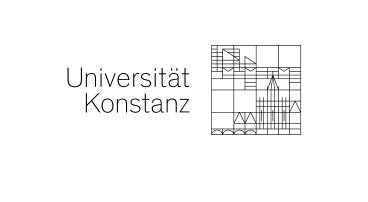
\includegraphics{konstanz-logo}\\
\vspace{20mm}
{\fontsize{12}{14.4} \selectfont
	Faculty of Humanities\\
	Department of Linguistics
}
\end{center}
\vfill{}
Konstanz, 2025
\newpage\mbox{}\thispagestyle{empty}

\newpage
\restoregeometry
\rmfamily
}
}

% Title and date

\title{This is my thesis}
\date{}
\begin{document}
\maketitle

%% LATEX CODE!
\linespread{1.5}
\pagenumbering{roman} % Ensure Roman numbering continues
\setcounter{page}{1}  % Reset page number to i

\chapter*{Abstract}\label{abstract}
Here!
% The abstract should outline the main approach and findings of the thesis and must not be more than 500 words.



\chapter*{Acknowledgements or Preface}\label{acknowledgements}


I am beyond grateful for my supervisors Bettina Braun and Tamara Rathcke for accompanying me.

as my mentor Katharina Zahner-Ritter

Thanks to the coffee-club four countless trips to the Campus Café and small breaks in the sun
Marieke and Svenja for Mittelbaustuff
Susan Reichelt for always being there, teaching, swimming,
peer PhDs and post-docs (Susan),

Schreibfaultiere Angela, Tianyi, Meike
Meike Rommel, Angela James, Tianyi Zhao, Hendrik Behrens-Zemek
Current and former members of AG Braun and the Babylab, especially Hendrik Behrens-Zemek, Friederike Hohl, Luisa Geib, Michelle Vuong, Naomi Reichmann
Katharina Hölzl for sharing the first year of this project

friends I acquired during my studies: Hannah, Linnea, Lisa, Marlena,

to my friends in Freiburg
My partner Felix, for always supporting and encouraging me
My friends and family at home and someplace in the world, for your willing to use Zoom after work, four countless game nights and stays over the weekend

for their help in recruiting their own friend's and family's kids

Julia and Peter with Emma and Mara


Tady \& Heiko

Adriana for being so patient


former freiburger colleagues, especially tobias streck, martin pfeiffer, elisabeth zima, göz kaufmann, adriana hanulikova, peter auer, johanna hantsch/masuch, maj-brit


project partner marie-anne morand
for help and testing in switzerlang marco bleiker + moritz daum

for making me feel welcome in Konstanz after spending so much time at University Freiburg

for all the lovely people I met on conferences, some of which became my friends.
For friends with kids, all families and kids taking part in our studies

DFG for funding

Linguistica initiated by Hanna Fischer
unite and bildet banden

tübinger for adopting me at conference trips Ulrike Schneider, Claudia Friedrichs, Jessica Steil

lettng me test: babylab potsdam (Tom, Natalie, Hiwis) + wortschatzinsel göttingen (Nivi, Christina


for my Rollerderby teammates in Freiburg who thought me the amount of frustration tolerance and endurance for my PhD
esp. Edda, Rebecca, Becksi, Kathrin L., Silke, Vicky, Ultra

friends who let me tag along during their phd

never felt to truly belong
arbeiterkind

to my family (my parents, siblings and grandparents half of which I lost along the way)

to believing in myself and trusting the process
I know I'm very privileged to have met you all along the way.
Thank you!


Thank you for accompanying me on my journey called life so far, it would not have been the same without you.

\renewcommand*\contentsname{Contents}
{
\setcounter{tocdepth}{1}
\tableofcontents
}
\listoffigures
\listoftables
\setstretch{1.5}
\bookmarksetup{startatroot}

\chapter*{Copyright notice}\label{copyright-notice}
\addcontentsline{toc}{chapter}{Copyright notice}

\markboth{Copyright notice}{Copyright notice}

Produced on 24 November 2024.

© Susan Su (2024).

\bookmarksetup{startatroot}

\chapter*{Abstract}\label{abstract}
\addcontentsline{toc}{chapter}{Abstract}

\markboth{Abstract}{Abstract}

The abstract should outline the main approach and findings of the thesis
and must not be more than 500 words.

\bookmarksetup{startatroot}

\chapter*{Declaration}\label{declaration}
\addcontentsline{toc}{chapter}{Declaration}

\markboth{Declaration}{Declaration}

\begin{quote}
Use only one of the following declarations (Standard thesis or Thesis
including published works declaration) and remove the other.
\end{quote}

\subsection*{Standard thesis}\label{standard-thesis}
\addcontentsline{toc}{subsection}{Standard thesis}

This thesis is an original work of my research and contains no material
which has been accepted for the award of any other degree or diploma at
any university or equivalent institution and that, to the best of my
knowledge and belief, this thesis contains no material previously
published or written by another person, except where due reference is
made in the text of the thesis.

Student name:

Student signature:

Date:

\subsubsection*{Publications during
enrolment}\label{publications-during-enrolment}
\addcontentsline{toc}{subsubsection}{Publications during enrolment}

\begin{quote}
Remove this section if you do not have publications.
\end{quote}

The material in Chapter~\ref{sec-intro} has been submitted to the
journal \emph{Journal of Impossible Results} for possible publication.

The contribution in Chapter~\ref{sec-litreview} of this thesis was
presented in the International Symposium on Nonsense held in Dublin,
Ireland, in July 2022.

\subsubsection*{Reproducibility
statement}\label{reproducibility-statement}
\addcontentsline{toc}{subsubsection}{Reproducibility statement}

This thesis is written using Quarto with renv (Ushey 2022) to create a
reproducible environment. All materials (including the data sets and
source files) required to reproduce this document can be found at the
Github repository
\href{https://github.com/SusanSu/thesis}{\texttt{github.com/SusanSu/thesis}}.

This work is licensed under a
\href{http://creativecommons.org/licenses/by-nc-sa/4.0/}{Creative
Commons Attribution-NonCommercial-ShareAlike 4.0 International License}.

\subsection*{Thesis including published works
declaration}\label{thesis-including-published-works-declaration}
\addcontentsline{toc}{subsection}{Thesis including published works
declaration}

I hereby declare that this thesis contains no material which has been
accepted for the award of any other degree or diploma at any university
or equivalent institution and that, to the best of my knowledge and
belief, this thesis contains no material previously published or written
by another person, except where due reference is made in the text of the
thesis.

This thesis includes ?? original papers published in peer reviewed
journals and ?? submitted publications. The core theme of the thesis is
??. The ideas, development and writing up of all the papers in the
thesis were the principal responsibility of myself, the student, working
within the Department of Econometrics \& Business Statistics under the
supervision of ??

(The inclusion of co-authors reflects the fact that the work came from
active collaboration between researchers and acknowledges input into
team-based research.)

In the case of (??insert chapter numbers) my contribution to the work
involved the following:

\begingroup\fontsize{10}{12}\selectfont

\resizebox{\ifdim\width>\linewidth\linewidth\else\width\fi}{!}{
\begin{tabu} to \linewidth {>{\raggedleft\arraybackslash}p{1.2cm}>{\raggedright\arraybackslash}p{2.6cm}>{\raggedright}X>{\raggedright\arraybackslash}p{2.6cm}>{\raggedright\arraybackslash}p{2.6cm}>{\raggedright\arraybackslash}p{2.6cm}}
\toprule
\multicolumn{1}{>{\raggedright\arraybackslash}p{1.2cm}}{\textbf{Thesis chapter}} & \multicolumn{1}{>{\raggedright\arraybackslash}p{2.6cm}}{\textbf{Publication title}} & \multicolumn{1}{l}{\textbf{Status}} & \multicolumn{1}{>{\raggedright\arraybackslash}p{2.6cm}}{\textbf{Nature and \% of student contribution}} & \multicolumn{1}{>{\raggedright\arraybackslash}p{2.6cm}}{\textbf{Nature and \% of coauthors' contribution}} & \multicolumn{1}{>{\raggedright\arraybackslash}p{2.6cm}}{\textbf{Coauthors are Monash students}}\\
\midrule
2 & The life cycle of Mongolian crickets & Submitted & Concept and data analysis, writing first draft: 60\% & Shu Xu, input into manuscript: 25\%; Eddie Betts, input into manuscript: 15\% & Shu Xu: No; Eddie Betts: Yes\\
\bottomrule
\end{tabu}}
\endgroup{}

I have / have not renumbered sections of submitted or published papers
in order to generate a consistent presentation within the thesis.

Student name:

Student signature:

Date:

I hereby certify that the above declaration correctly reflects the
nature and extent of the student's and co-authors' contributions to this
work. In instances where I am not the responsible author I have
consulted with the responsible author to agree on the respective
contributions of the authors.

Main Supervisor name:

Main Supervisor signature:

Date:

\bookmarksetup{startatroot}

\chapter*{Acknowledgements}\label{acknowledgements}
\addcontentsline{toc}{chapter}{Acknowledgements}

\markboth{Acknowledgements}{Acknowledgements}

I would like to thank my pet goldfish for \ldots{}

\begin{quote}
In accordance with Chapter 7.1.4 of the research degrees handbook, if
you have engaged the services of a~professional~editor, you
must~provide~their name~and a brief description of the service rendered.
If the professional editor's current or former area of academic
specialisation is similar your own, this too should be stated as it may
suggest to examiners that the editor's advice to the student has
extended beyond guidance on English expression to affect the substance
and structure of the thesis.
\end{quote}

\begin{quote}
If you have used generative artificial intelligence (AI) technologies,
you must include a written acknowledgment of the use and its extent.
Your acknowledgement should at a minimum specify which technology was
used, include explicit description on how the information was generated,
and explain how the output was used in your work. Below is a suggested
format:
\end{quote}

\begin{quote}
``I acknowledge the use of {[}insert AI system(s) and link{]} to
{[}specific use of generative artificial intelligence{]}. The output
from these was used to {[}explain use{]}.''
\end{quote}

\begin{quote}
Free text section for you to record your acknowledgment and gratitude
for the more general academic input and support such as financial
support from grants and scholarships and the non-academic support you
have received during the course of your enrolment. If you are a
recipient of the ``Australian Government Research Training Program
Scholarship'', you are required to include the following statement:
\end{quote}

\begin{quote}
\begin{quote}
``This research was supported by an Australian Government Research
Training Program (RTP) Scholarship.''
\end{quote}
\end{quote}

\begin{quote}
You may also wish to acknowledge significant and substantial
contribution made by others to the research, work and writing
represented and/or reported in the thesis. These could include
significant contributions to: the conception and design of the project;
non-routine technical work; analysis and interpretation of research
data; drafting significant parts of the work or critically revising it
so as to contribute to the interpretation.
\end{quote}

\clearpage\pagenumbering{arabic}\setcounter{page}{1}

\bookmarksetup{startatroot}

\chapter{Introduction}\label{sec-intro}

This is where you introduce the main ideas of your thesis, and an
overview of the context and background.

In a PhD, Chapter 2 would normally contain a literature review.
Typically, Chapters 3--5 would contain your own contributions. Think of
each of these as potential papers to be submitted to journals. Finally,
Chapter 6 provides some concluding remarks, discussion, ideas for future
research, and so on. Appendixes can contain additional material that
don't fit into any chapters, but that you want to put on record. For
example, additional tables, output, etc.

\section{Quarto}\label{quarto}

In this template, the rest of the chapter shows how to use quarto. The
big advantage of using quarto is that it allows you to include your R or
Python code directly into your thesis, to ensure there are no errors in
copying and pasting, and that everything is reproducible. It also helps
you stay better organized.

For details on using Quarto, see \url{http://quarto.org}.

\section{Data}\label{data}

Included in this template is a file called \texttt{sales.csv}. This
contains quarterly data on Sales and Advertising budget for a small
company over the period 1981--2005. It also contains the GDP (gross
domestic product) over the same period. All series have been adjusted
for inflation. We can load in this data set using the following code:

\begin{Shaded}
\begin{Highlighting}[]
\NormalTok{sales }\OtherTok{\textless{}{-}}\NormalTok{ readr}\SpecialCharTok{::}\FunctionTok{read\_csv}\NormalTok{(here}\SpecialCharTok{::}\FunctionTok{here}\NormalTok{(}\StringTok{"data/sales.csv"}\NormalTok{)) }\SpecialCharTok{|\textgreater{}}
  \FunctionTok{rename}\NormalTok{(}\AttributeTok{Quarter =} \StringTok{\textasciigrave{}}\AttributeTok{...1}\StringTok{\textasciigrave{}}\NormalTok{) }\SpecialCharTok{|\textgreater{}}
  \FunctionTok{mutate}\NormalTok{(}
    \AttributeTok{Quarter =} \FunctionTok{as.Date}\NormalTok{(}\FunctionTok{paste0}\NormalTok{(}\StringTok{"01{-}"}\NormalTok{, Quarter), }\StringTok{"\%d{-}\%b{-}\%y"}\NormalTok{),}
    \AttributeTok{Quarter =} \FunctionTok{yearquarter}\NormalTok{(Quarter)}
\NormalTok{  ) }\SpecialCharTok{|\textgreater{}}
  \FunctionTok{as\_tsibble}\NormalTok{(}\AttributeTok{index =}\NormalTok{ Quarter)}
\end{Highlighting}
\end{Shaded}

Any data you use in your thesis can go into the \texttt{data} directory.
The data should be in exactly the format you obtained it. Do no editing
or manipulation of the data prior to including it in the \texttt{data}
directory. Any data munging should be scripted and form part of your
thesis files (possibly hidden in the output).

\section{Figures}\label{figures}

Figure~\ref{fig-deaths} shows time plots of the data we just loaded.
Notice how figure captions and references work. Chunk names can be used
as figure labels with \texttt{fig-} prefixed. Never manually type figure
numbers, as they can change when you add or delete figures. This way,
the figure numbering is always correct.

\begin{figure}

\centering{

\includegraphics{01-chap1_files/figure-pdf/fig-deaths-1.pdf}

}

\caption{\label{fig-deaths}Quarterly sales, advertising and GDP data.}

\end{figure}%

\section{Results from analyses}\label{results-from-analyses}

We can fit a regression model to the sales data.

If \(y_t\) denotes the sales in quarter \(t\), \(x_t\) denotes the
corresponding advertising budget and \(z_t\) denotes the GDP, then the
resulting model is: \begin{equation}\phantomsection\label{eq-drm}{
  y_t = \beta x_t + \gamma z_t + \varepsilon_t
}\end{equation} where \(\hat{\beta} = 1.85\), and
\(\hat{\gamma} = 1.04\). We can reference this equation using
Equation~\ref{eq-drm}.

\section{Tables}\label{tables}

We can also make a nice summary table of the coefficients, as shown in
Table~\ref{tbl-coef}

\begin{longtable}[]{@{}lrr@{}}

\caption{\label{tbl-coef}Coefficients from the fitted model.}

\tabularnewline

\toprule\noalign{}
Coefficient & Estimate & P value \\
\midrule\noalign{}
\endhead
\bottomrule\noalign{}
\endlastfoot
(Intercept) & -438.98 & 0.02 \\
GDP & 1.04 & 0.02 \\
AdBudget & 1.85 & 0.00 \\

\end{longtable}

Again, notice the use of labels and references to automatically generate
table numbers.

\bookmarksetup{startatroot}

\chapter{Literature Review}\label{sec-litreview}

This chapter contains a summary of the context in which your research is
set.

Imagine you are writing for your fellow PhD students. Topics that are
well-known to them do not have to be included here. But things that they
may not know about should be included.

Resist the temptation to discuss everything you've read in the last few
years. And you are not writing a textbook either. This chapter is meant
to provide the background necessary to understand the material in
subsequent chapters. Stick to that.

You will need to organize the literature review around themes, and
within each theme provide a story explaining the development of ideas to
date. In each theme, you should get to the point where your ideas will
fit in. But leave your ideas to later chapters. This way it is clear
what has been done beforehand, and what new contributions you are making
to the research field.

All citations should be done using markdown notation as shown below.
This way, your bibliography will be compiled automatically and
correctly.

\section{Exponential smoothing}\label{sec-expsmooth}

Exponential smoothing methods were originally developed in the late
1950s (Brown 1959, 1963; Holt 1957; Winters 1960). Because of their
computational simplicity and interpretability, they became widely used
in practice.

Empirical studies by Makridakis and Hibon (1979) and Makridakis et al.
(1982) found little difference in forecast accuracy between exponential
smoothing and ARIMA models. This made the family of exponential
smoothing procedures an attractive proposition (see Chatfield et al.
2001).

The methods were less popular in academic circles until Ord et al.
(1997) introduced a state space formulation of some of the methods,
which was extended in Hyndman et al. (2002) to cover the full range of
exponential smoothing methods.

\bookmarksetup{startatroot}

\chapter*{Bibliography}\label{bibliography}
\addcontentsline{toc}{chapter}{Bibliography}

\markboth{Bibliography}{Bibliography}

\phantomsection\label{refs}
\begin{CSLReferences}{1}{0}
\bibitem[\citeproctext]{ref-Brown59}
Brown, R. G. (1959), \emph{Statistical forecasting for inventory
control}, McGraw-Hill, New York.

\bibitem[\citeproctext]{ref-Brown63}
Brown, R. G. (1963), \emph{Smoothing, forecasting and prediction of
discrete time series}, Englewood Cliffs, New Jersey: Prentice Hall.

\bibitem[\citeproctext]{ref-CKOS01}
Chatfield, C., Koehler, A. B., Ord, J. K., and Snyder, R. D. (2001),
{``A new look at models for exponential smoothing,''} \emph{The
Statistician}, 50, 147--159.

\bibitem[\citeproctext]{ref-Holt57}
Holt, C. E. (1957), \emph{Forecasting trends and seasonals by
exponentially weighted averages}, O.N.R. Memorandum, Carnegie Institute
of Technology.

\bibitem[\citeproctext]{ref-HKSG02}
Hyndman, R. J., Koehler, A. B., Snyder, R. D., and Grose, S. (2002),
{``A state space framework for automatic forecasting using exponential
smoothing methods,''} \emph{International Journal of Forecasting}, 18,
439--454.

\bibitem[\citeproctext]{ref-M1comp}
Makridakis, S., Anderson, A., Carbone, R., Fildes, R., Hibon, M.,
Newton, R. L. J., Parzen, E., and Winkler, R. (1982), {``The accuracy of
extrapolation (time series) methods: Results of a forecasting
competition,''} \emph{Journal of Forecasting}, 1, 111--153.

\bibitem[\citeproctext]{ref-MH79}
Makridakis, S., and Hibon, M. (1979), {``Accuracy of forecasting: An
empirical investigation (with discussion),''} \emph{Journal of Royal
Statistical Society (A)}, 142, 97--145.

\bibitem[\citeproctext]{ref-OKS97}
Ord, J. K., Koehler, A. B., and Snyder, R. D. (1997), {``Estimation and
prediction for a class of dynamic nonlinear statistical models,''}
\emph{Journal of American Statistical Association}, 92, 1621--1629.

\bibitem[\citeproctext]{ref-renv}
Ushey, K. (2022),
\emph{\href{https://CRAN.R-project.org/package=renv}{{renv}: Project
environments}}.

\bibitem[\citeproctext]{ref-Winters60}
Winters, P. R. (1960), {``Forecasting sales by exponentially weighted
moving averages,''} \emph{Management Science}, 6, 324--342.

\end{CSLReferences}



\end{document}
